\subsubsection{Complex step differentiation and forward AD: dealing with epsilons}

Notice that both AD based on dual number and complex-step differentiation introduce an abstract unit ($\epsilon$ and $i$, respectively) associated with the imaginary part of the extender value that carries forward the numerical value of the gradient.
% This resemblance between the methods makes them susceptible to the same advantages and disadvantages: easiness of implementation with operator overloading; and inefficient scaling with respect to the number of variables to differentiate. 
Although these methods seem similar, we emphasize that AD gives the exact gradient, whereas complex step differentiation relies on numerical approximations that are valid only when the stepsize $\varepsilon$ is small. 
In Figure \ref{fig:complex-step-AD} we show how the calculation of the gradient of $\sin (x^2)$ is performed by these two methods.
Whereas the second component of the dual number has the exact derivative of the function $\sin(x^2)$ with respect to $x$, it is not until we take $\varepsilon \rightarrow 0$ that we obtain the derivative in the imaginary component for the complex step method.
% The stepsize dependence of the complex step differentiation method makes it resemble more to finite differences than AD with dual numbers. 
The dependence of the complex step differentiation method on the step size gives it a closer resemblance to finite difference methods than to AD using dual numbers.
Further notice the complex step method involves more terms in the calculation, a consequence of the fact that second order terms of the form $i^2 = -1$ are transferred to the real part of the complex number, while for dual numbers the terms associated to $\epsilon^2 = 0$ vanish. 
\begin{figure}[t]
    \centering
    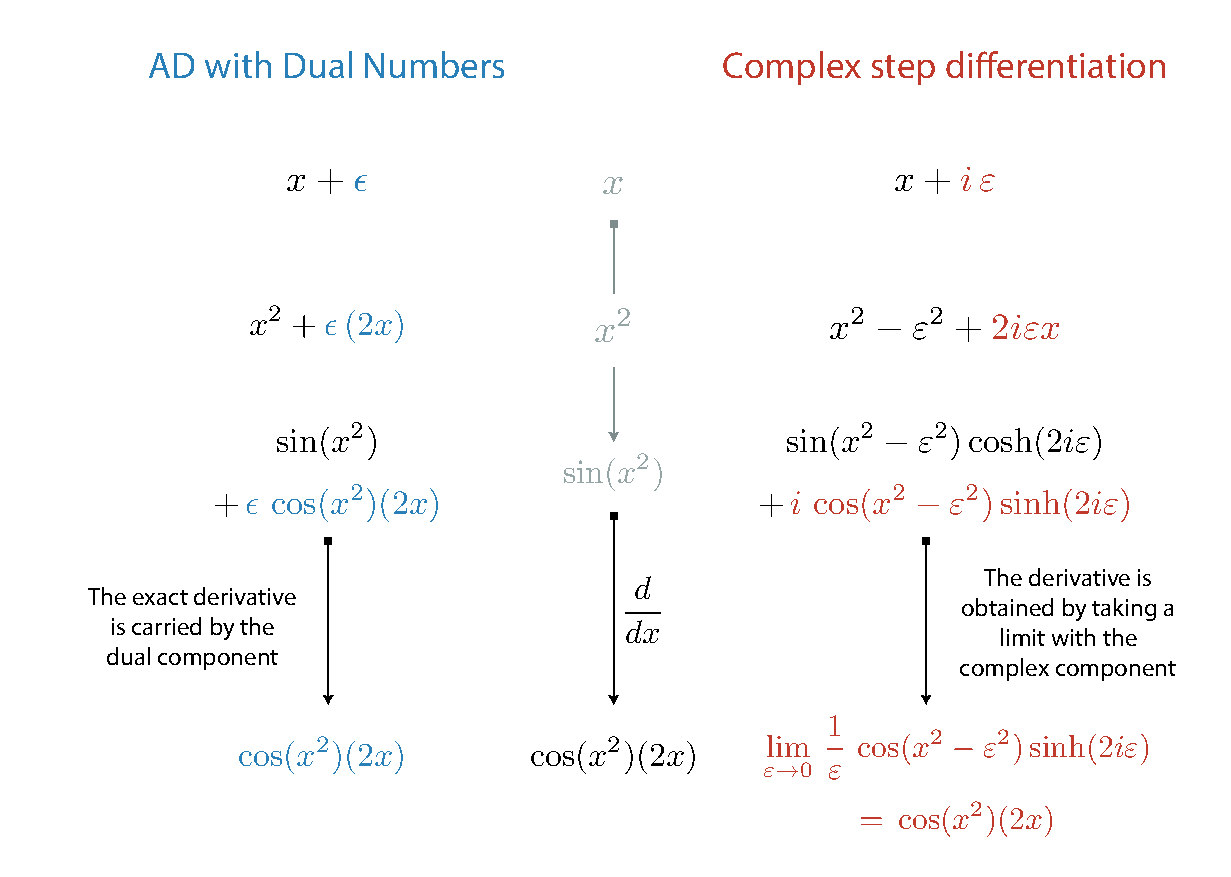
\includegraphics[width=0.75\textwidth]{tex/figures/complex-step-AD.pdf}
    \caption{Comparison between AD implemented with dual numbers and complex step differentiation. For the simple case of the function $f(x) = \sin(x^2)$, we can see how each operation is carried in the forward step by the dual component (blue) and the complex component (red). Whereas AD gives the exact gradient at the end of the forward run, in the case of the complex step method we need to take the limit in the imaginary part. }
    \label{fig:complex-step-AD}
\end{figure}

% \subsubsection{Forward and backwards AD: connection with JVPs and VJPs}

\subsubsection{Forward AD and sensitivity equations: solving for the sensitivity}

The sensitivity equations can also be solved in discrete forward mode by numerically discretizing the original ODE and later deriving the discrete sensitivity equations \cite{ma2021comparison}. 
For most cases, this leads to the same result than in the continuous case \cite{FATODE2014}.
% To illustrate this, consider the simple forward Euler method applied to the original ODE given by $u_{t+1} = u_t + \Delta t \, f(u_t, \theta, t)$.
We can numerically solve for the sensitivity $s$ by extending the parameter $\theta$ to a multidimensional dual number %\cite{Neuenhofen_2018, RevelsLubinPapamarkou2016}, 
\begin{equation}
    \theta =
    \begin{bmatrix}
    \theta_1 \\
    \theta_2 \\
    \vdots \\
    \theta_p
    \end{bmatrix}
    \rightarrow
    \begin{bmatrix}
    \theta_1 + \epsilon_1 \\
    \theta_2 + \epsilon_2 \\
    \vdots \\
    \theta_p + \epsilon_p
    \end{bmatrix}
\end{equation}
where $\epsilon_i \epsilon_j = 0$ for all pairs of $i$ and $j$ (see Section \ref{section:dual-numbers}). 
The dependency of the solution $u$ of the ODE on the parameter $\theta$ is now expanded following Equation \eqref{eq:dual-number-function} as 
\begin{equation}
    u =
    \begin{bmatrix}
    u_1 \\
    u_2 \\
    \vdots \\
    u_n
    \end{bmatrix}
    \rightarrow
    \begin{bmatrix}
    u_1 + \sum_{j=1}^p \frac{\partial u_1}{\partial \theta_j} \epsilon_j \\
    u_2 + \sum_{j=1}^p \frac{\partial u_2}{\partial \theta_j} \epsilon_j \\
    \vdots \\
    u_p + \sum_{j=1}^p \frac{\partial u_n}{\partial \theta_j} \epsilon_j
    \end{bmatrix}
    = 
    u \, + \, s \, 
    \begin{bmatrix}
    \epsilon_1 \\
    \epsilon_2 \\
    \vdots \\
    \epsilon_p
    \end{bmatrix},
\end{equation}
that is, the dual component of the vector $u$ corresponds exactly to the sensitivity matrix $s$. 
This implies forward AD applied to any multistep linear solver will result in the application of the same solver to the sensitivity equations \eqref{eq:sensitivity_equations}.  
For example, for the forward Euler method this gives 
\begin{align}
    u^{t+1} + \epsilon \, s^{t+1}
    &= 
    u^t + \epsilon \, u^t + \Delta t \, f (u^t + \epsilon \, s^t, \theta + \epsilon, t) \nonumber \\
    &= 
    u^t + f(u^t, \theta, t) 
    + 
    \epsilon \, \Delta t 
    \left( 
    \frac{\partial f}{\partial u} s^t + 
    \frac{\partial f}{\partial \theta}
    \right).
    \label{eq:sensitivity-equation-AD}
\end{align}
The dual component corresponds to the forward Euler discretization of the sensitivity equation \eqref{eq:sensitivity_equations}, with $s^t$ the temporal discretization of the sensitivity $s(t)$.
For non-linear numerical solver (e.g., Runge-Kutta methods), the discretization forward AD will lead to a different numerical solver for the sensitivity.  

\subsubsection{Discrete adjoints vs backwards AD}
\label{section:comparison-discrete-adjoint-AD}

??
% Is the adjoint the same than a gradient? Yes, but these are derivatives with respect to the state of the system, not with respect to the parameters! 

\subsubsection{Discrete vs continuous adjoints}

% There is a large family of adjoint methods that in first order can be classified as discrete and continuous adjoints. 
As previously mentioned, the difference between the discrete and continuous adjoint methods is that the former follows the discretize-then-differentiate approach (also known as finite difference of adjoints \cite{Sirkes_Tziperman_1997}).
In contrast, continuous adjoint equations are derived by directly operating on the differential equation, without a priori consideration of the numerical scheme used to solve it. 
In some sense then, we can think of the discrete adjoint $\lambda = (\lambda_1, \lambda_2, \ldots, \lambda_N)$ in Equation \eqref{eq:linea-adjoint-state-equation} as the discretization of the continuous adjoint $\lambda(t)$. 

A natural question then is if these two methods effectively compute the same gradient, i.e., if the discrete adjoint consistently approximate its continuous counterpart. 
Different works exist regarding the consistency or inconsistency between the two approaches, and this usually depends on the ODE and equation.  
Proofs of the consistency of discrete adjoint methods for Runge-Kutta methods have been provided in \cite{sandu2006properties, sandu2011solution}.
Depending on the choice of the Runge-Kutta coefficients, we can have a numerical scheme that is both consistent for the original equation and consistent/inconsistent for the adjoint \cite{Hager_2000}.
Furthermore, adjoint methods can fail in chaotic systems \cite{Wang2012-chaos-adjoint}.

In the more general case, both methods can give different computational results \cite{Sirkes_Tziperman_1997}.
It has been shown \cite{Sirkes_Tziperman_1997} that discrete adjoints can lead to instabilites and wrong gradients.